Although a finished panel was not part of the formal project scope, the full design process was carried out to simulate the complete production cycle of a Eurorack module. 
Eurorack panels are typically manufactured from \qty{2}{mm} anodised aluminium \cite{ConstructionDetailsA100}. 
Panel graphics are commonly applied via UV printing directly onto the anodised surface 
-- a process that offers fine detail, and 
resistance to scratching and UV exposure \cite{FrontPanelExpressa}. 
The following section briefly describes the process from CAD modelling and prototype verification through to photorealistic rendering for product presentation.

\paragraph{CAD}

The physical front panel was designed in FreeCAD, modelling the mechanical constraints of the Eurorack format, described in 
Section~\ref{sec:eurorack-fundamentals}: \qty{10}{HP} (\qty{50.80}{mm}) wide -- to fit the underlying PCB width a width of \qty{46}{mm} -- and \qty{128.5}{mm} tall, with 4 M3 mounting holes in the corners.

\begin{wrapfigure}{r}{0.5\textwidth}
	\centering
	\vspace{-1em}
	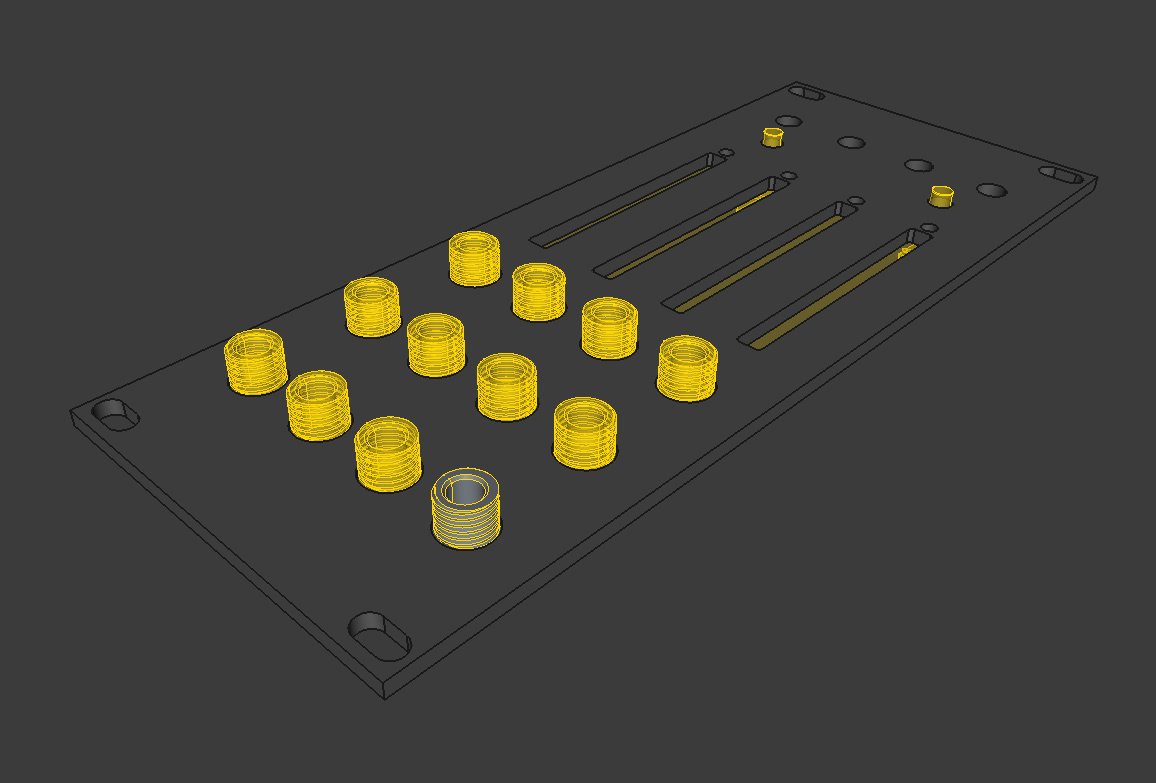
\includegraphics[width=0.48\textwidth]{../images/panel_design/panel_freecad.png}
	\caption{CAD model of Panel in FreeCAD -- with highlighted ShapeBinders}
	\vspace{-1.0em}
	\label{fig:panel_freecad}
\end{wrapfigure}

The panel cutout positions were imported directly from the KiCad PCB layout using the KiCad StepUp workbench plugin for FreeCAD, which imports the KiCad board as a 3D assembly with all component positions preserved. 

Within FreeCAD, \textit{ShapeBinders} \cite{PartDesignShapeBinder2025} were used to reference the imported component geometries directly -- the cutout dimensions and positions in the panel sketch are parametrically constrained to the STL geometry of each component interfering with the frontpanel. 

Figure \ref{fig:panel_freecad} shows the highlighted parts that needed to be cut out in FreeCAD. 

\paragraph{3D Print Verification}

Before committing to a final aluminum panel, the design was verified by 3D printing the panel. 
The printed panel fit the components and mounted into the Eurorack rack correctly on the first attempt, confirming that the 
KiCad StepUp import and ShapeBinder workflow produced accurate dimensions without any manual measurements and correction. 
The 3D printed panel also served as a functional prototype for evaluating the physical layout and ergonomics of the controls before the final panel is produced.

%TODO insert photo

\paragraph{Graphic Design}

The mechanical outline was exported from FreeCAD as a technical drawing, on form of a .dxf file, providing an exact 1:1 scale template for the panel artwork. 
The DXF was imported into Inkscape as a locked base layer, and the panel graphics -- labels, module name, signal flow indicators -- were designed on top. 
Exporting the finished artwork as SVG preserves full vector fidelity, making it suitable for handoff to a graphic designer or direct submission to a panel manufacturer.

\begin{figure}[H]
	\centering
	\begin{minipage}{0.3\textwidth}
		\centering
		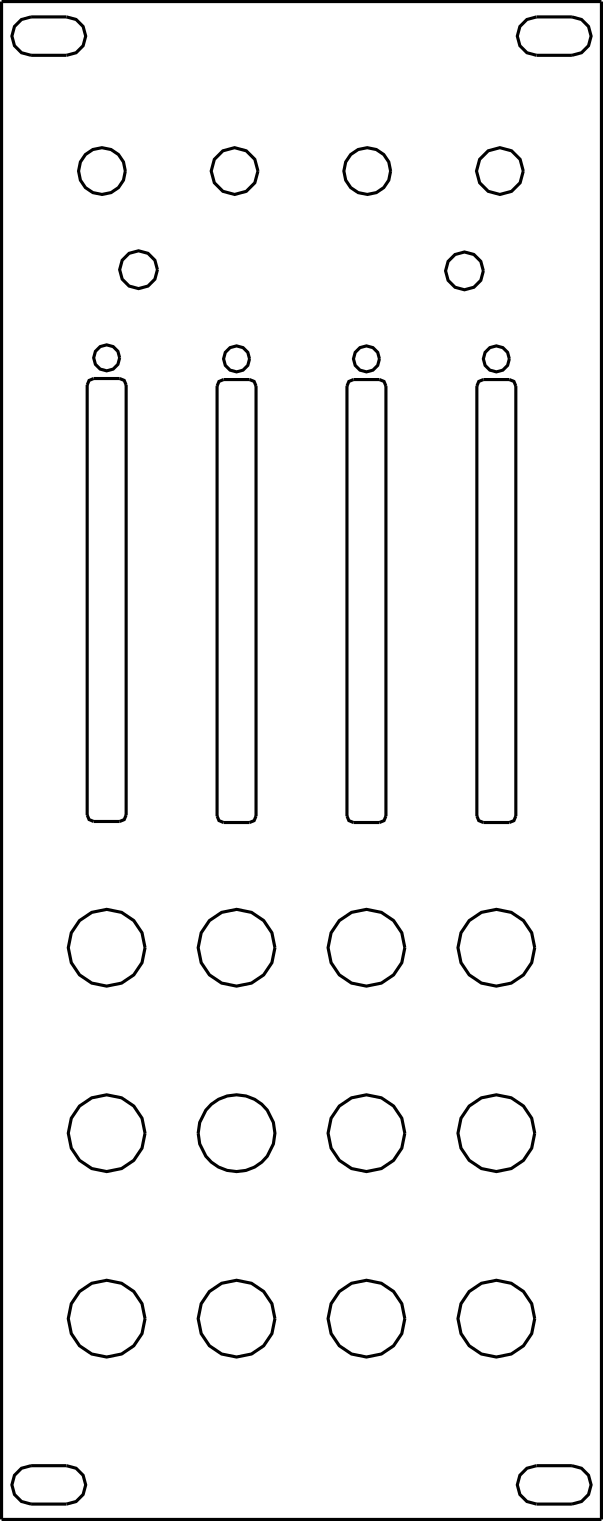
\includegraphics[width=0.5\textwidth]{../images/panel_design/panel_svg_outlines_only.png}
		\subcaption{Drill and cut outline for aluminium panel}
	\end{minipage}
	\hfill
	\begin{minipage}{0.3\textwidth}
		\centering
		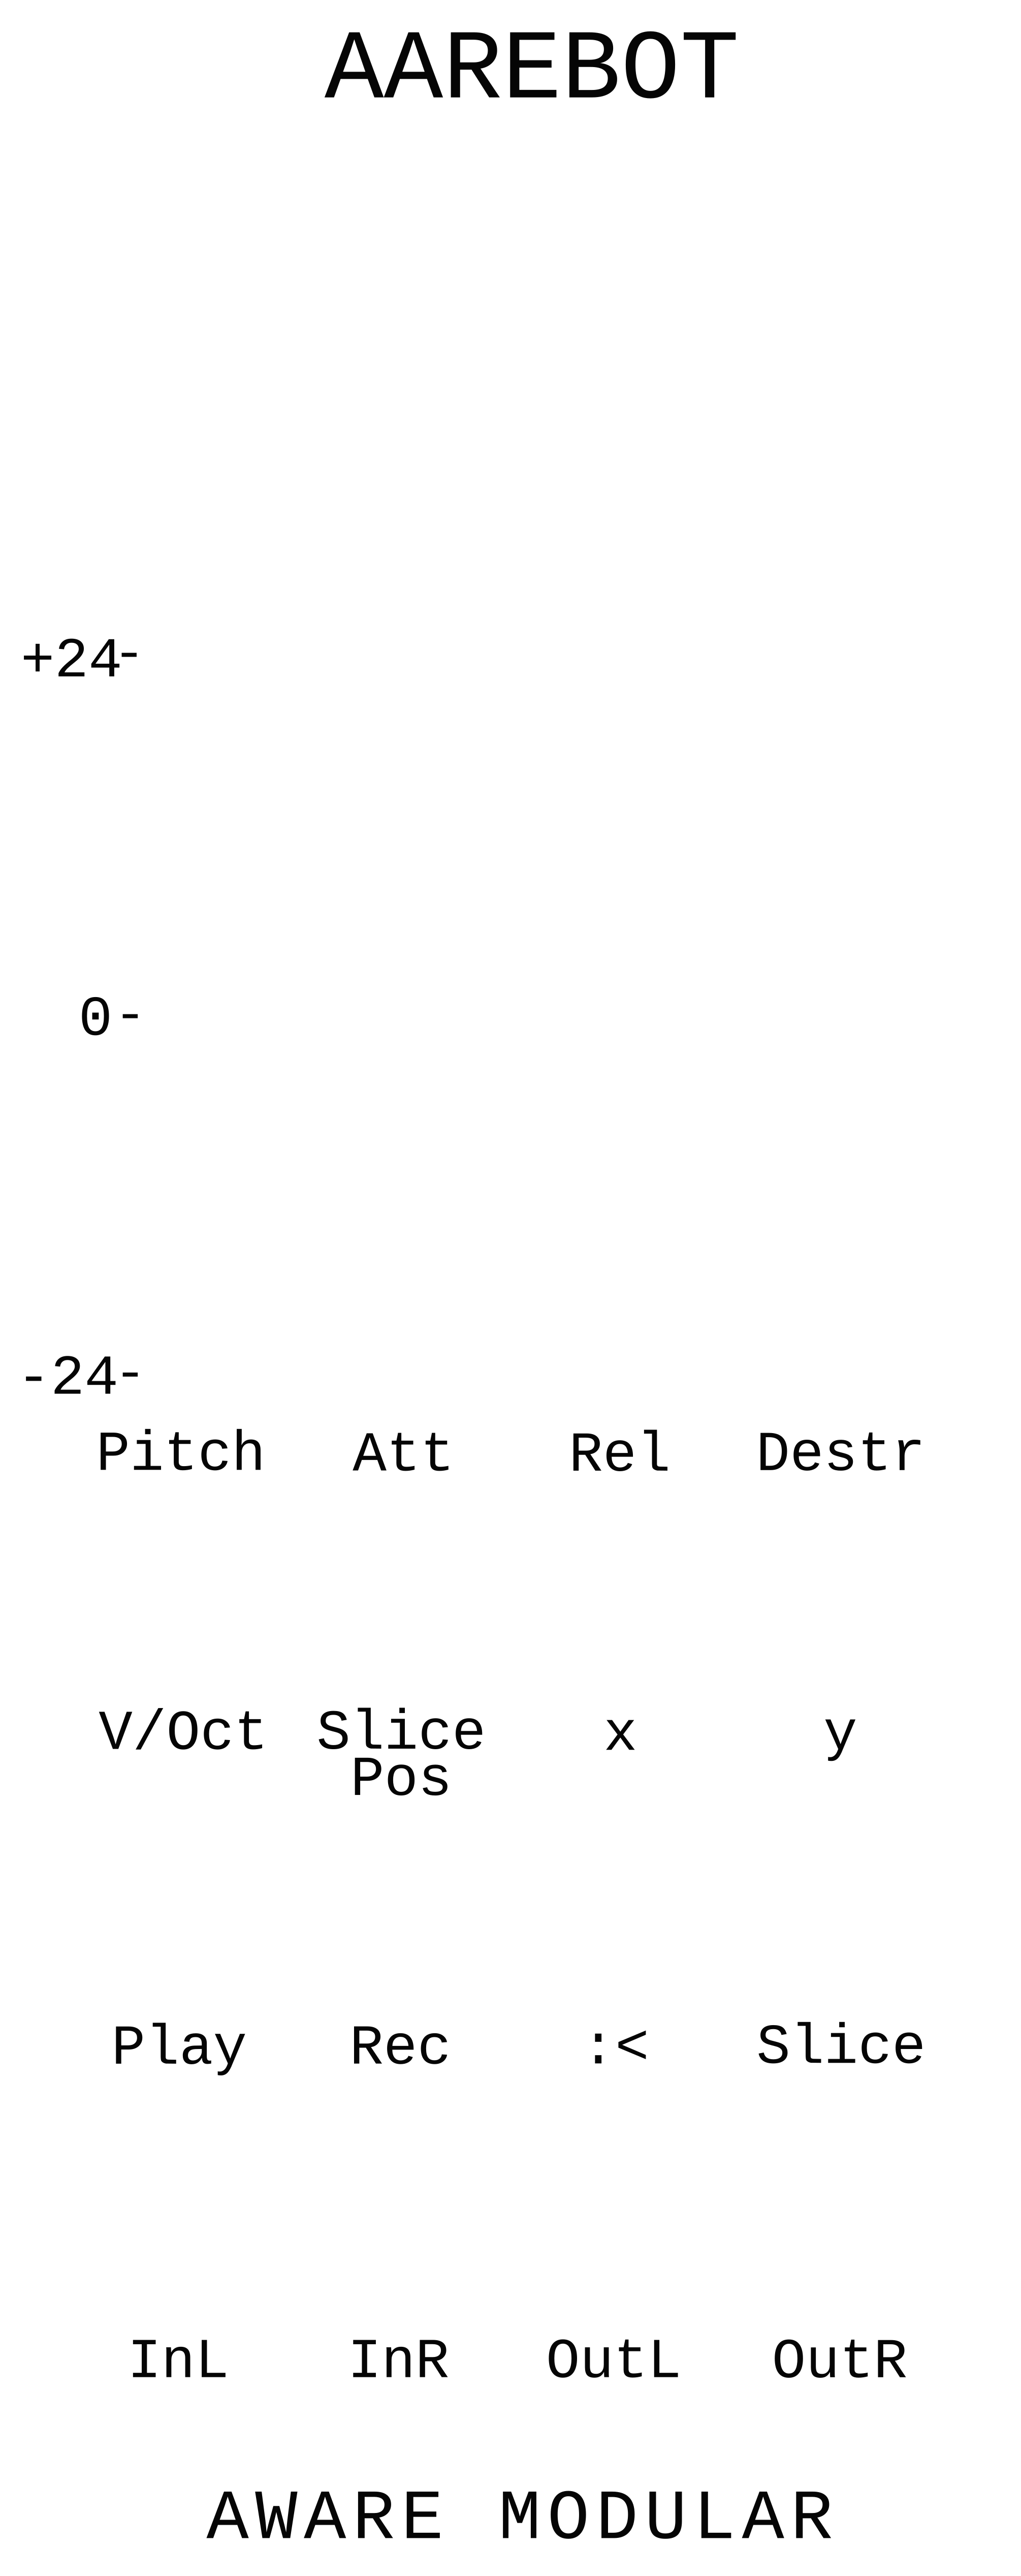
\includegraphics[width=0.5\textwidth]{../images/panel_design/panel_svg_design_only.png}
		\subcaption{Graphic design layer}
	\end{minipage}
	\hfill
	\begin{minipage}{0.3\textwidth}
		\centering
		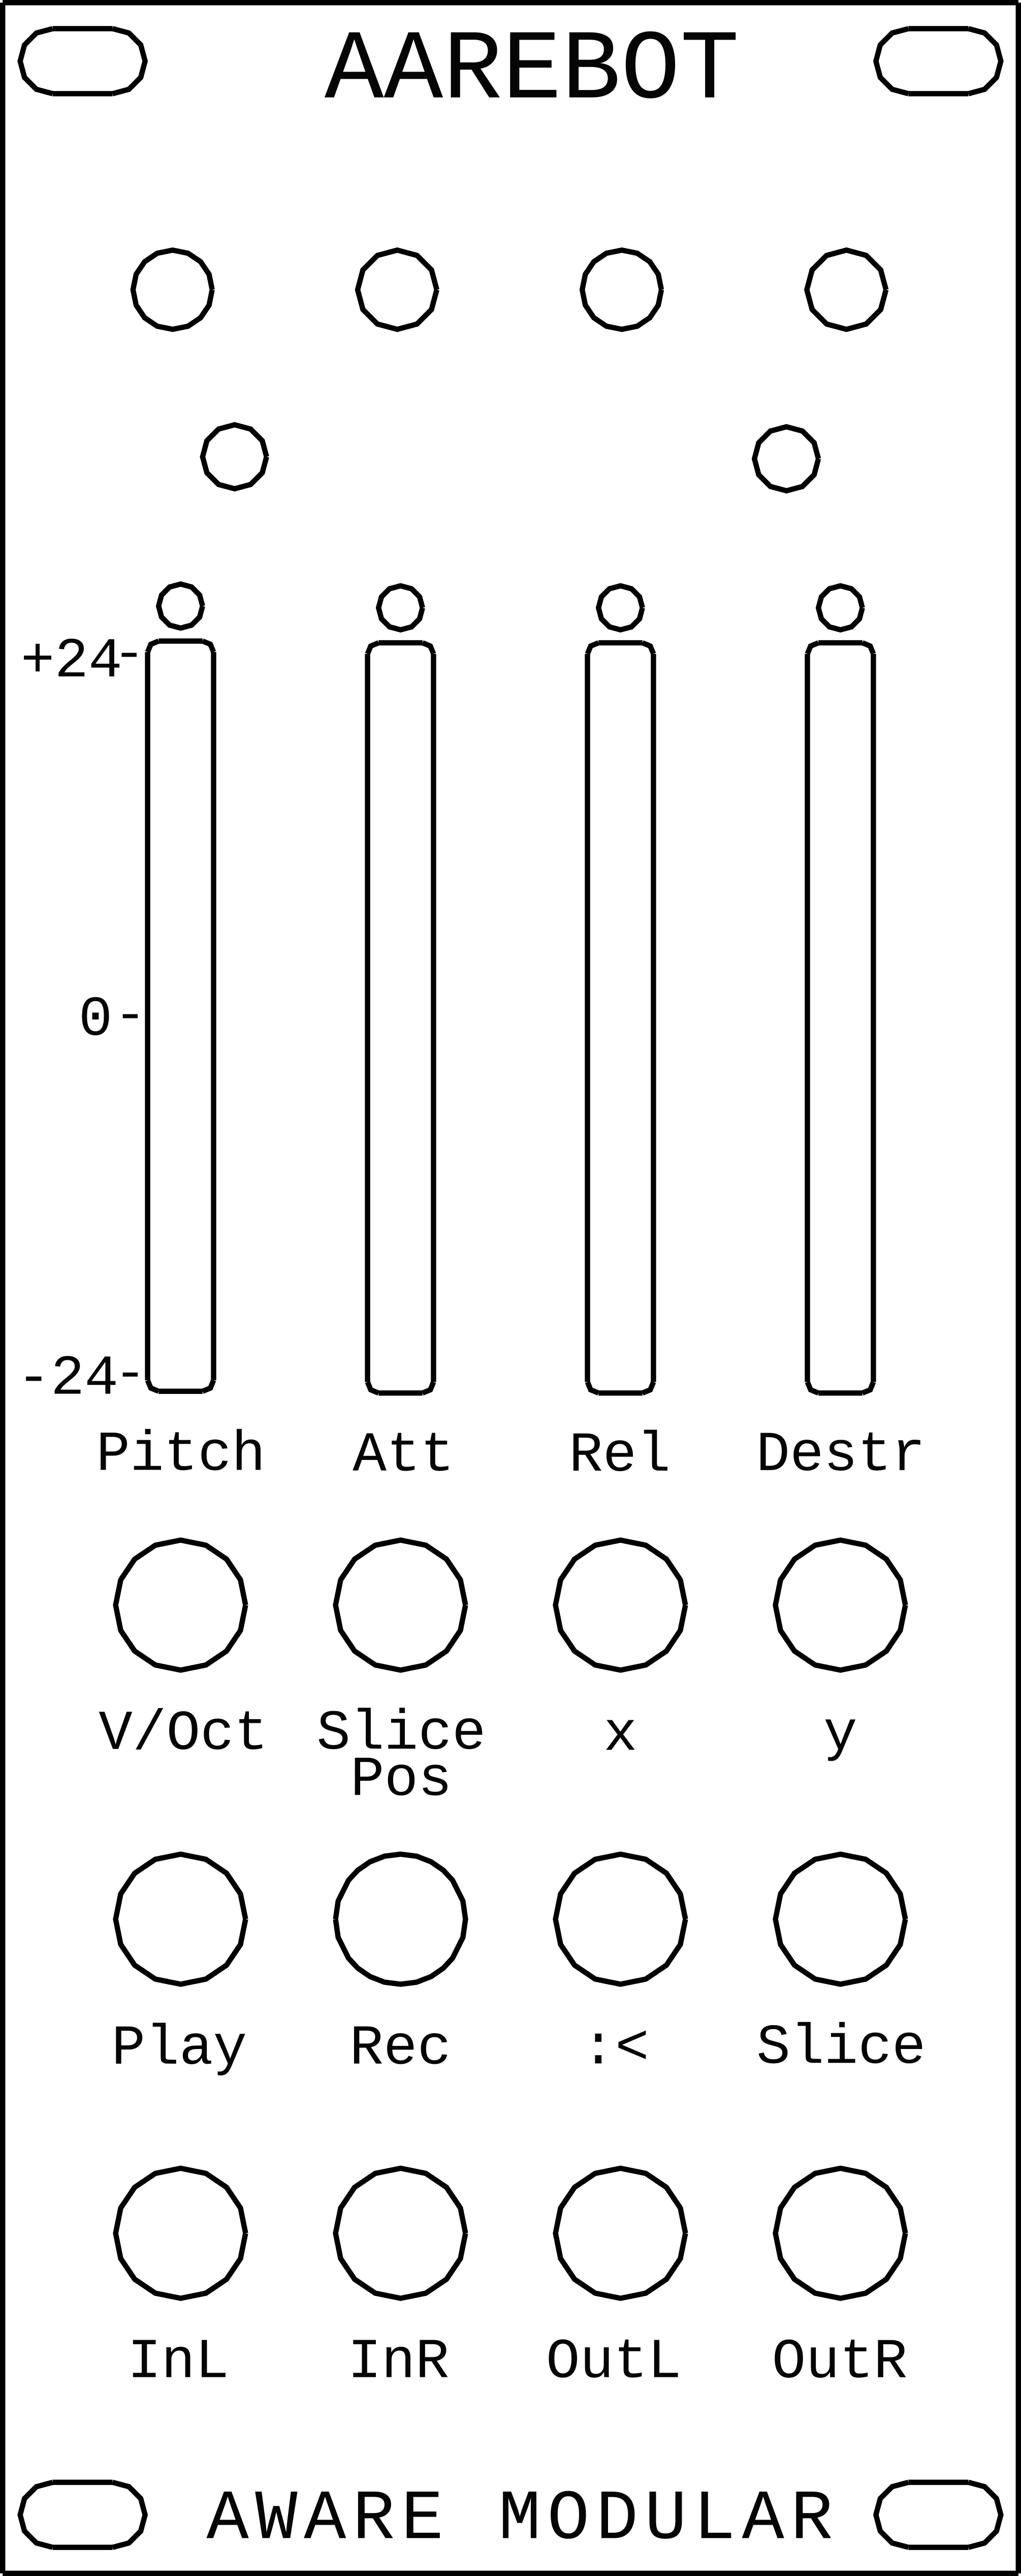
\includegraphics[width=0.5\textwidth]{../images/panel_design/panel_svg_design_and_outlines.png}
		\subcaption{Combined}
	\end{minipage}
	\caption{Panel SVG design workflow in Inkscape.}
	\label{fig:panel_svg}
\end{figure}


\paragraph{3D Rendering}

For product presentation -- including the title page image and the module overview in Section~\ref{sec:high-level-system-overview} -- the panel was rendered in Blender. 
The FreeCAD model was exported as an OBJ file, which Blender imports natively. 
The finished panel artwork was exported from Inkscape as a high-resolution PNG and applied as a texture on the panel face using Blender's Principled BSDF material.

Tailored materials and light sources were added to show LED colors and improve visual fidelity. 
The scene was rendered using Cycles with a brushed aluminium material on the panel body.

\begin{figure}[H]
	\centering
	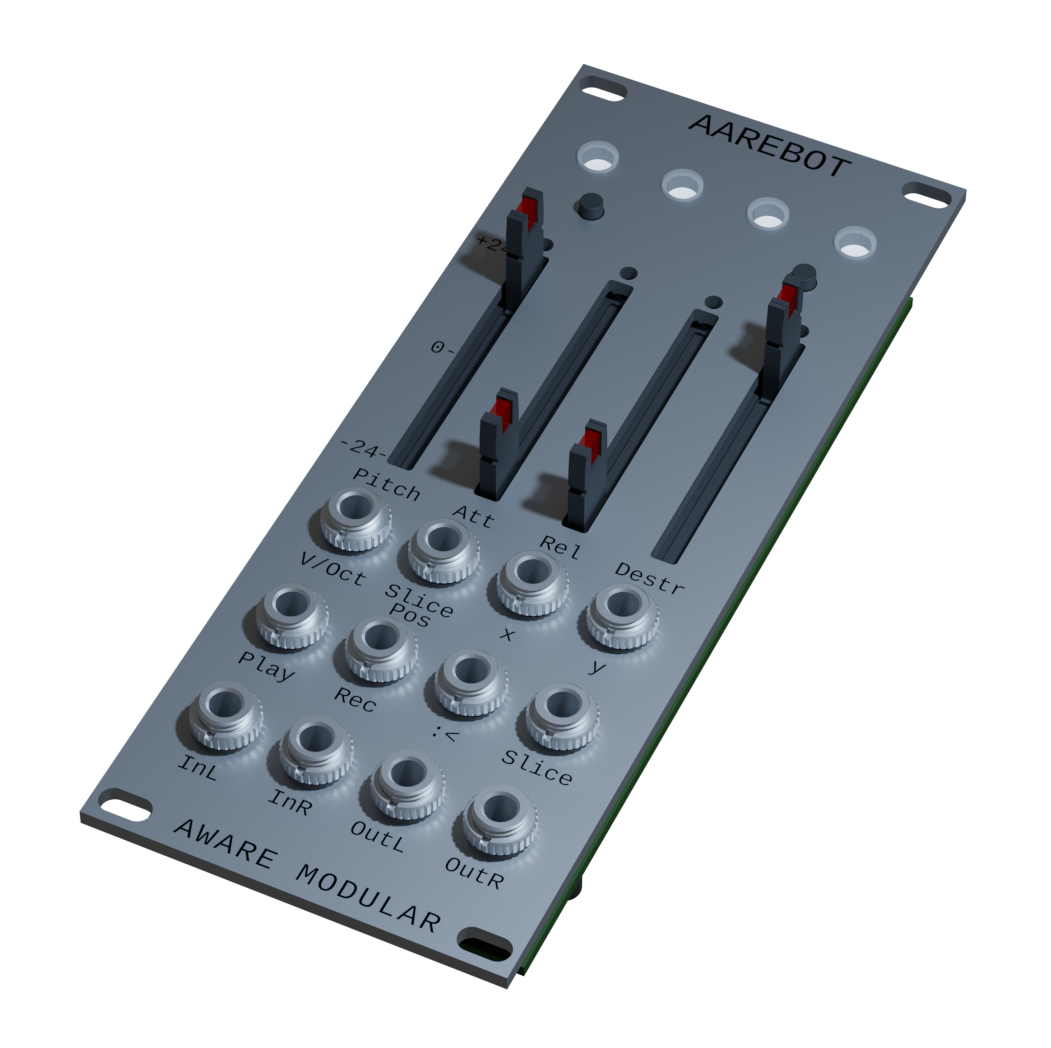
\includegraphics[width=0.4\textwidth]{../../images/aarebot_render_20260316_cropped.png}
	\caption{Blender render of the finished module panel.}
	\label{fig:panel_render}
\end{figure}

This workflow -- mechanical CAD in FreeCAD, graphic design in Inkscape, and photorealistic rendering in Blender -- allowed a complete product design cycle to be carried out using open-source tools while producing both manufacturing-ready files and presentation-quality visuals within the scope of this project.